\section{Rupture Optimizations}\label{subsec:optimizations}

\subsection{Block alignment}\label{subsec:blockalign}
Block ciphers are \textit{length monotonic}, but not \textit{strictly length
monotonic}, as described in section \ref{subsec:lenmonotone}. Specifically, the
length of the encrypted text is rounded up to a product of $\mu$-bits, where
$\mu$ is the block size. This results in plaintext length difference between two
messages not always resulting in length difference between the respective
encrypted ciphertext.

We bypass this problem by using block alignment techniques
\cite{moller2014poodle}. This method demands issuing multiple requests to the
reflection oracle while including artificial noise.  In each request $r_{i, c}$
for each candidate $c$ in the secret alphabet, we add increasing artificial
noise. That way, all $r_{1, c}$ for the candidates will contain one
character of alignment noise, $r_{2, c}$ two characters and so forth.
Therefore, for some alignment noise length $a \in [0, \mu)$ the reflection
of the correct candidate will be $(\delta*\mu)$ and for all incorrect
candidates $(\delta*\mu)+1$. In that case, the incorrect candidates result
in one more block compared to the correct one. This ensures that one out of
$\ceil{\mu / |r_i|}$ requests will result in a block distinction between the
alphabet candidates. Figure \ref{fig:block_alignment} depicts the block
alignment technique intuitively.

   \begin{figure}[thpb]
      \centering
          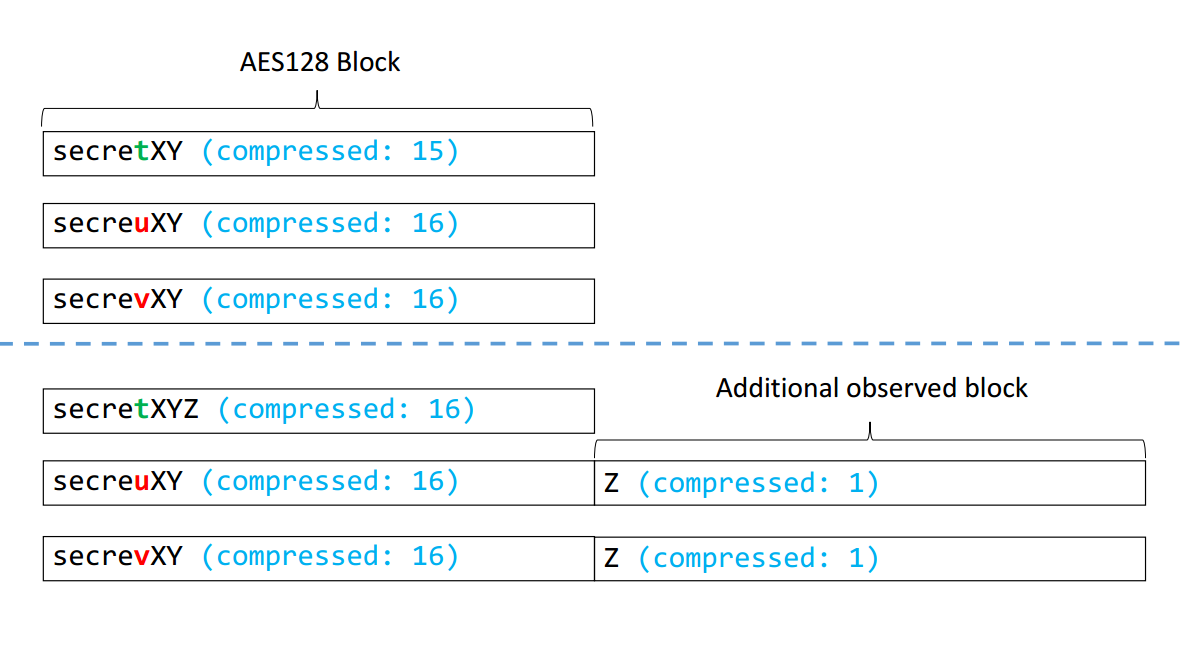
\includegraphics[width=0.48\textwidth]{figures/block_alignment.png}
      \caption{The block alignment method}
      \label{fig:block_alignment}
   \end{figure}

\subsection{Reflection computation methods}\label{subsec:reflectionmethods}
The reflection strings $r$ should be polynomially computable, as defined in
\ref{subsec:propertycom}. BREACH is parameterized with an alphabet of ASCII
symbols $\Sigma$ for each character of the secret and a successful attack should
distinguish a single character of the alphabet through a series of requests.

The first method of issuing these requests is serial. Each request contains to a
single character of the alphabet and an attack phase is completed when requests
have been issued for the entire alphabet. The complexity of this attack is
$\mathcal{O}(|\Sigma|)$ and the round ends by finding a character of the secret.
This method is similar to how BREACH previously worked.

The second method of attack is divide and conquer. In each phase the alphabet is
divided into two subsets $\Sigma_1$ and $\Sigma_2 = \Sigma \setminus \Sigma_1$,
where $|\Sigma_1| = |\Sigma_2| = \ceil{|\Sigma| / 2}$. The reflection string for
$\Sigma_1$ consists of $|\Sigma_1|$ substrings separated by an annotation symbol
$\beta$.  Each substring consists of the known prefix concatenated with a
candidate in $\Sigma_1$.  For example, if $\Sigma_1$ is $\{"1", "2"\}$ and the
known prefix is "abc", using "-" as $\beta$ the reflection is: "abc1-abc2". The
reflection string for $\Sigma_2$ is constructed similarly.

As long as the prefix of the secret is \textit{compression-detectable} by each
substring of the reflection, the end of each phase marks the choice of subset
$\Sigma_i$ that contains the correct alphabet symbol.  When $|\Sigma| = 1$ the
round is complete. Each round reduces the alphabet by half, so the complexity of
this attack is $\mathcal{O}(log|\Sigma|)$. Figure \ref{fig:divide_and_conquer}
depicts the reflection sequence for the case when the alphabet consists of
number digits.

   \begin{figure}[thpb]
      \centering
          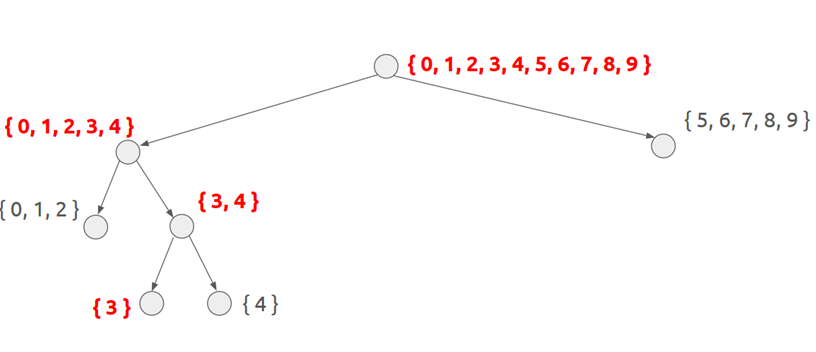
\includegraphics[width=0.48\textwidth]{figures/divide_and_conquer.png}
      \caption{The divide \& conquer method}
      \label{fig:divide_and_conquer}
   \end{figure}

\subsection{Request parallelization}\label{subsec:parallel}
The reflection oracle is generally synchronous, although it may be able to
handle multiple parallel requests from the adversary.  This is the case in
BREACH.  Modern web servers are able to handle multiple parallel requests and
browsers can issue a certain amount of parallel requests per domain. This
functionality enables the adversary to issue multiple parallel requests per
symbol in alphabet $\Sigma$ and efficiently reduce the execution time of the
attack.

\subsection{Request soup}
Previous sections demonstrated the need for multiple requests per reflection
string $r_i$. However, communication with the reflection oracle is time
expensive, so it may be preferable to issue multiple requests for a candidate
and treat them as a set rather than separately.

This technique is useful in the case of BREACH. A request set consists of
requests for a symbol $s_i$ in alphabet $\Sigma$. Bigger request sets result in
less time delay and the adversary can measure the mean length over the number of
requests in the set.
